\section {Previous Work}
As sir Isaac Newton once said: "If I have seen further it is only by standing on the shoulders of giants." No academic research can be done single handedly. The first part of this section will give a short summary of what has been researched earlier within, or related to, the ROLE-project. These topics include the personal learning environments, widgets and the psycho-pedagogical integration model. The second part will give an introduction to the methods and tools used in this thesis. These topics include interaction design and the use of personas.

\subsection { Personal Learning Environments }
A personal learning environment (PLE) is not an application. A PLE consists of different tools and services used in everyday learning \cite{attwell}. A PLE is as the name suggests personal. In a class of 30 students it is likely to find 30 different learning environments. A common set up is a word processor, a web browser, a mail client and a communication tool. The web browser probably displays multiple web sites including searches for academic research, tools for quickly checking facts and a translating service. All of these programs and websites take a lot of place on the screen, it also takes time to set up. There is also no guarantee that these programs work well together.  It might be preferable if all these tools could be incorporated into one larger system with set standards for synchronizing tools with each other.

Looking at the requirements from the ROLE-project (The full list can be found in the requirements section, section 3.1) we find the following requirements: “ROLE should provide users with the ability to construct and maintain a Personal Learning Environment. (PLE)” and “Inter-tool communication in the PLE” \cite{chatterjee}. This means that the experimental platform PLESpaces should allow students to create a personal learning environment where the tools added should be able to communicate with each other. Within the ROLE-project it has been decided to build systems, like PLESpaces, as a widget space where individual widgets, with widget-communication capabilities, can be added.

A special feature called recommendation service should also be included. This service should analyse the user's behaviour, such as current goals and previous knowledge, and deliver recommendations. These recommendations include tools, complete widget spaces and fellow students for collaboration.

\subsection {Widgets}
Widget is an ambiguous term. The definition according to Cambridge Advanced Learner's Dictionary is  "any small device whose name you have forgotten or do not know" or "an imagined small product made by a company".
In today's world of IT widgets often refer to a small single purpose application that can be attached to a widget area. Widgets are used in systems like Apple's Macintosh Dashboard, Gadgets in Microsoft's Windows Vista and Windows 7 and mobile platforms such as Google's Android. In the ROLE-project and this thesis widgets refers to "small portable Web-enabled applications" that can be run in a web environment. \cite{kiefel}

\subsubsection {OpenApp}
Widgets are allowed to communicate with each other. If an action occurs in one widget (e.g the user makes a selection) another widget could activate and react accordingly (e.g. save information as a bookmark). Within the ROLE-project a framework called OpenApps has been developed \cite{isaksson}. This framework defines how widgets send and receive messages to and from other widgets.

\subsubsection {Widget Space}
Inspired by Google's system iGoogle the ROLE-project has developed the idea that widgets should be added to domain specific widget spaces. iGoogle is a service meant as a start page for web browsers. The user can add widgets to this start page in order to access information and activities without leaving the start page. \cite{igoogle} The widget spaces in a system like PLESpaces could be different courses or parts of a course \cite{palmer}. One idea is that everyone can create spaces. Each of these spaces should have a specific purpose. The creator of a widget space adds widgets to the widget space and then invites users to share the space with \cite {kiefel}.

\subsection {Psycho-Pedagogical Integration Model}
The Psycho-Pedagogical Integration Model (PPIM) tries to identify how learning is best achieved. PPIM is based on the concept of self regulated learning. The main idea is that learning a specific area is divided into phases where the student plans, learns and reflect. PPIM divides the students' work into four phases: \cite {nussbaumer}
\begin {enumerate}
	\item Learner profile model is defined or revised
	\item Learner finds and selects learning resources
	\item Learner works on selected learning resources
	\item Learner reflects and reacts on strategies goals
\end {enumerate}

The following paragraphs are short summaries of each of the phases in the psycho-pedagogical integration model.

\subsubsection {Learner profile model is defined or revised}
This is where goals and sub-goals are defined. Info such as previous knowledge of the field and history of how learning was achieved is also taken into account. As a last step system settings are added to finalize the student's profile for the current learning domain.

Here the ROLE-project suggests that the personalized learning environment (PLE) should be able to react to the profile and make suitable recommendations. The student's profile is updated by the student (by self evaluation and reflection), by the PLE (by tracking and monitoring tools) and also by tutors and teachers. From the profile the experimental platform should give recommendations of for example students with similar goals for cooperation.

\subsubsection {Learner finds and selects learning resources}
This phase focuses on the gathering of learning material. In this context learning material includes traditional study material such as books and articles, but also tools in the PLE. Learning resources could also include students with the same goals.

In this phase the PLE should give recommendations of such learning material. Recommendations should be based on the profile created in the previous phase. The student should also be able to interact with other students and teachers to share and receive resources. At the end it should always be up to the student to choose his or her learning material.

\subsubsection {Learner works on selected learning resources}
This is the traditional learning phase. The student work with the chosen resources to complete the goals set in phase one. During this phase the PLE should encourage the student to perform self-assessment and allow external assessment through other students and teachers. The information from the assessments will be transferred to the next phase where reflection will take place. It is up to the student to decide if assessments from other parts should be included in the next phase or not.

\subsubsection {Learner reflects and reacts on strategies goals}
When the traditional learning is completed the student is supposed to reflect on the work done. Were the goals achieved? How were they achieved? Was the strategy efficient?
The experimental platform should be able to assist the student in this reflection. The student then choose which of the reflections should be transferred to the first stage to update the learning profile.

\subsection {Personas}
Personas are fictional characters who represent a certain group of users. These fictional characters are often accompanied by a use case scenario where the needs of the represented user group in the particular scenario is identified. Since these personas are not real users extensive research is needed to ensure these personas reflect the intended user group \cite{gudjonsdottir}. These personas are used as replacement users in phases where the intended users are not reachable. This can be due to practical reasons, such as geographical spread or time constraints.

Personas are given a name, age, occupation and sometimes even a picture, the picture can be animated or a real photo. The goal of a persona is to make it as lively as possible. When reading a persona's description and the following scenario it should be fairly logical that the persona reacts in a certain way. One way to create personas is to follow guides and check lists. One guide proposed these steps for creating a persona, in this case named Alan \cite{pruitt}.

\begin {itemize}
\item Get to know Alan, his business and family
\item Follow Alan through a typical day
\item Look at Alan's job description and role at work.
\item Get information about what Alan does when he’s not at work.
\item Understand the concerns Alan has about his life, career, and business.
\item Learn about Alan’s computer experience.
\item Understand the impact people like Alan have on our business.
\item Read key demographic information about Alan and his family.
\item Get a sense of what Alan does with technology.
\item Review Alan’s perspective on technology, past and future.
\item Learn how Alan keeps in touch with people.
\item Find out what Alan is like outside the U.S.
\item Hear what Alan has to say.
\end {itemize}

\subsection {Usability and Interaction Design}
This part will give a short introduction as to what usability and interaction design is. Tools will be presented that will aid the analysis of existing designs and the creation of new ones.

Usability is a term which is widely used today. When it comes to defining usability one is often directed to the phrase set by the International Organizations for Standardization (ISO): "The extent to which a product can be used by specified users to achieve specified goals with effectiveness, efficiency and satisfaction in a specified context of use".\cite{iso9241} Usability is, according to the ISO, contextual, meaning a usable system is only usable in the context for which is was designed. The ISO standard specifies ways of evaluating usability and defining the context of use, but it does not specify how to achieve a high level of usability.

Interaction design is one way of achieving high usability in a system. Interaction design is as the name suggests about designing for interaction. "Interaction design is an essential approach to the design of interactive systems" \cite{tinauli}. The idea is that IT-systems should be designed with the users' interaction in mind. Interaction design is sometimes connected to user-experience design and graphical design. The main difference is that interaction design focuses on the use and purpose of the program, where user-experience design and graphical design focuses on the experience and looks of the program.

One common way of creating systems for easy use it to make sure it follows the ten rules of heuristics \cite{nielsen}.

\begin {enumerate}
	\item Simple and natural dialogue.
	\item Speak the users' language.
	\item Minimize the users' memory load.
	\item Consistency.
	\item Feedback.
	\item Clearly marked exits.
	\item Shortcuts.
	\item Good error messages.
	\item Prevent errors.
	\item Help and documentation.
\end {enumerate}

\subsubsection {Previous Designs}
The following sketches have been developed by Uppsala Learning Lab. The sketches are evaluated in section 4.1. These sketches are quite similar to sketches developed at other universities within the ROLE-project. This is to be expected since the ROLE-project, like many other EU-projects, is also about sharing ideas and collaboration between countries.
\pagebreak
\begin{figure}[h]
	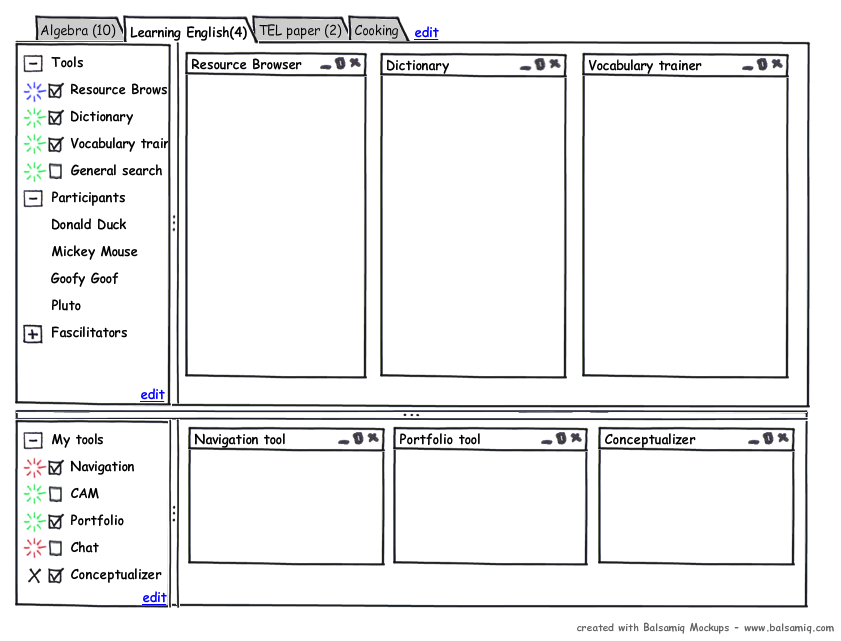
\includegraphics[width=1.0\textwidth] {uu_1.png}
	\caption {First draft from Uppsala Learning Lab}
	\label {fig:uu_1}
\end{figure}

In the first first draft the work space is divided into two areas; one course-related (top) and one personal (bottom). Both areas have a navigation area on the left hand side were tools can be opened or closed by checking or unchecking the box. New widgets can be added and existing widgets can be removed by clicking the edit-link at the bottom of the navigation area. At the top the student can choose which course to work with by changing tab. The student can also create new personal spaces. In this example there is a personal space called Cooking. These personal spaces are not to be confused with the personal area at the bottom part of the screen. On the left hand side you can activate and deactivate the tools for both the personal area and the workspace. Each tool has a coloured icon to the left which shows when widget-communications has been initiated and received. 

\pagebreak
The second version is based on the first sketch but with a few improvements. This version is a working system where widgets can be used to test the concept.
\begin{figure}[h!]
	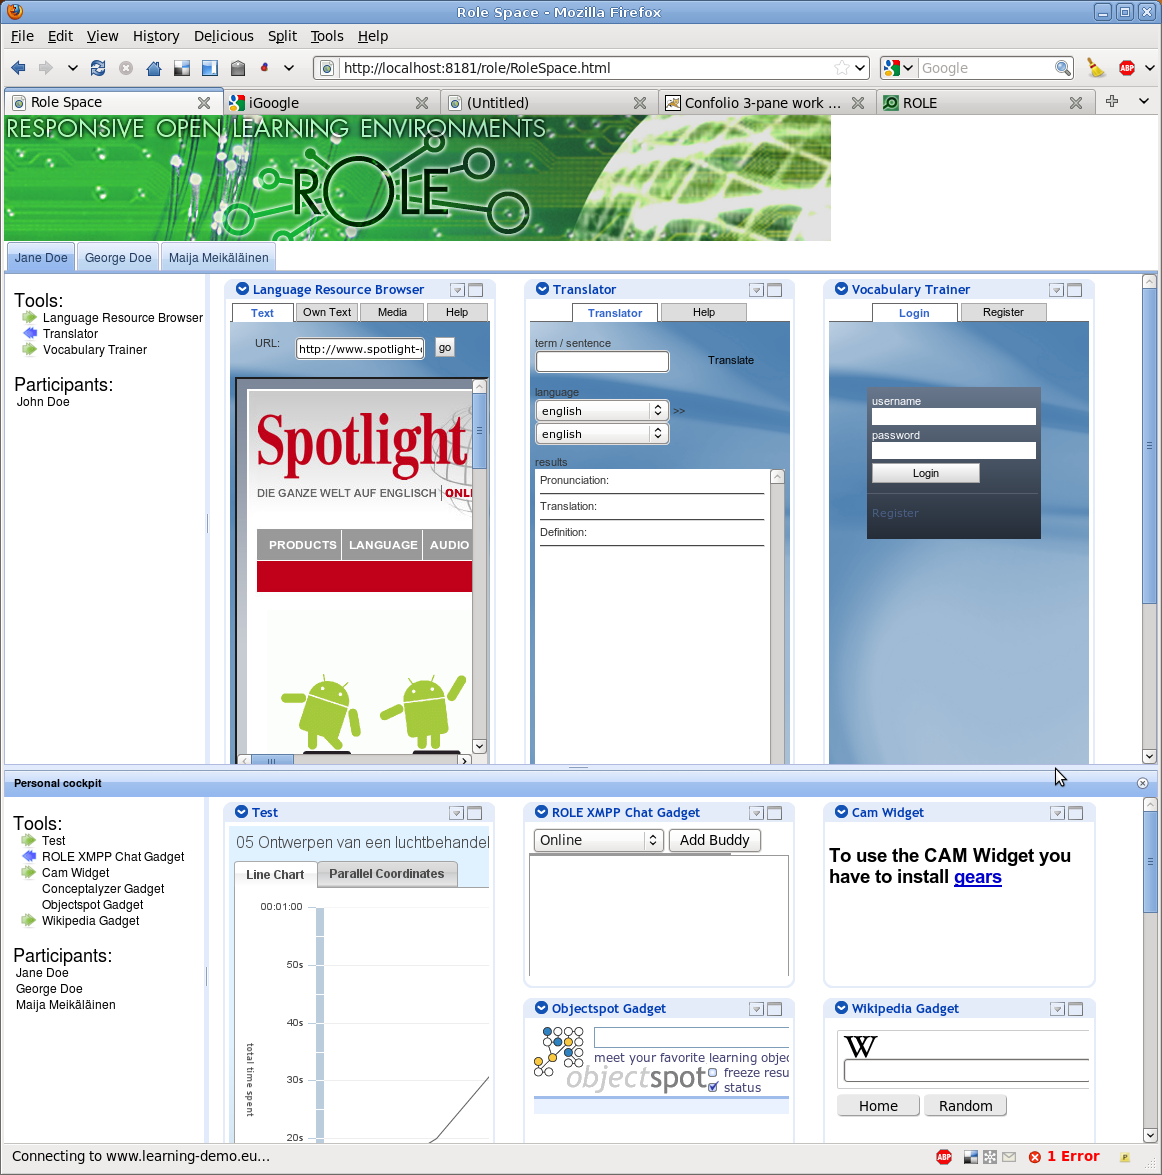
\includegraphics[width=1.0\textwidth] {uu_2.png}
	\caption {Second draft from Uppsala Learning Lab}
	\label {fig:uu_2}
\end{figure}

The major improvement here is in the navigation area on the left hand side. The change of activity icons to arrows clearly shows if an event has been sent or received. The use of shapes, instead of colours only, should help colour blind students. 

\pagebreak
The third version is also a working version. This is an early screen shot of the current version being developed at Uppsala Learning Lab.
\begin{figure}[h!]
	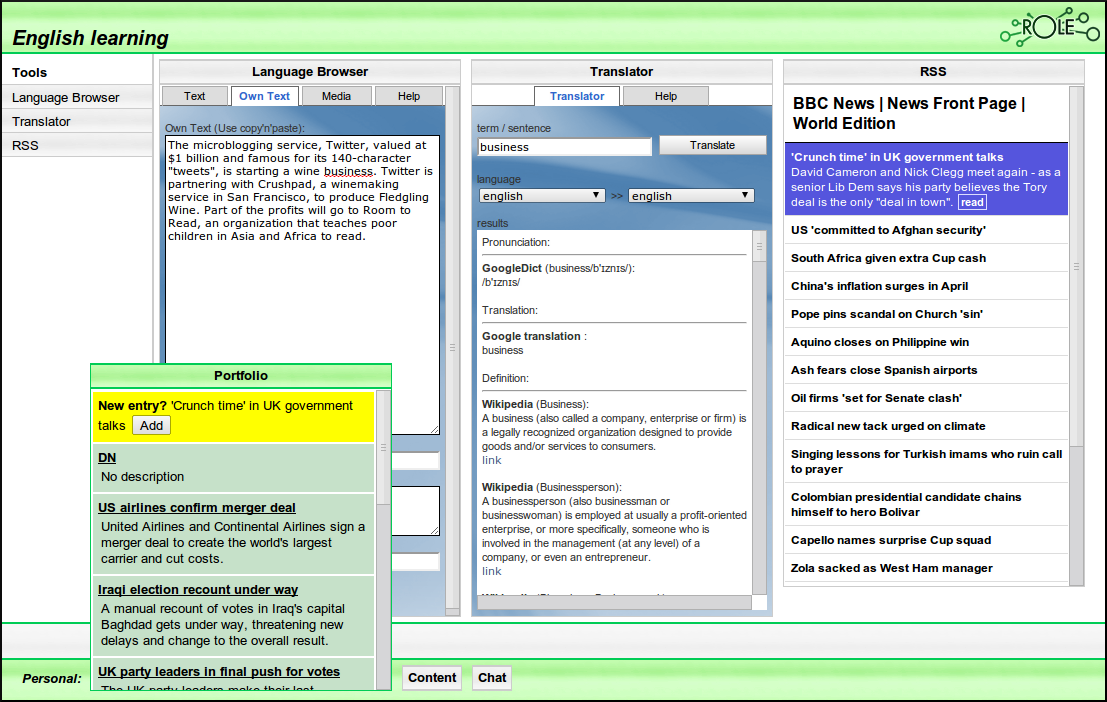
\includegraphics[width=1.0\textwidth] {uu_3.png}
	\caption {Third draft from Uppsala Learning Lab}
	\label {fig:uu_3}
\end{figure}

In this version the personal area has been minimized to a toolbar where the personal widgets will pop up when used. The icons for sending and receiving widget communications have also been removed. The main work area is larger, allowing for either bigger and more readable widgets, or more widgets allowing for easier multitasking. Another change is that different spaces is no longer visible by tabs at the top.
